
\begin{frame}{Slide for perfectionists}{how many word-breaks are}\relax
    \centering
    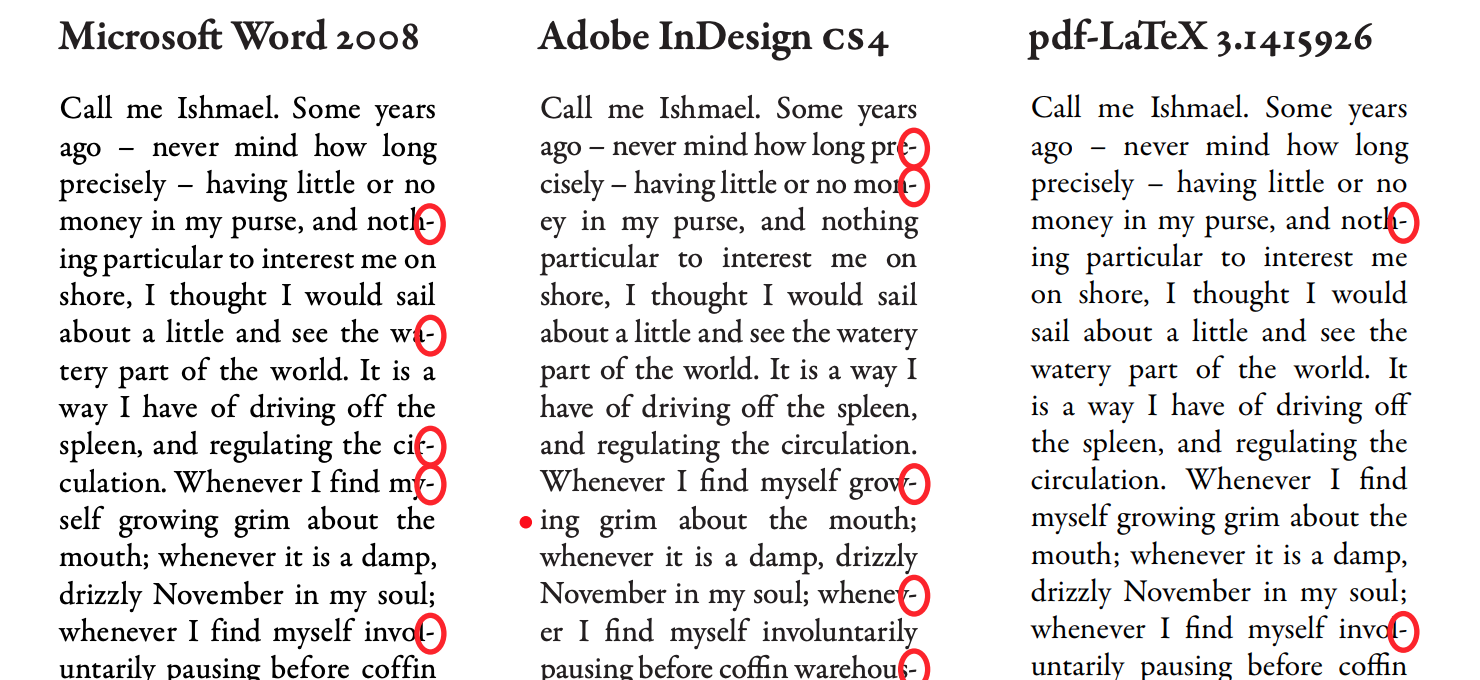
\includegraphics[width=0.6\textwidth]{twcomp}
    
    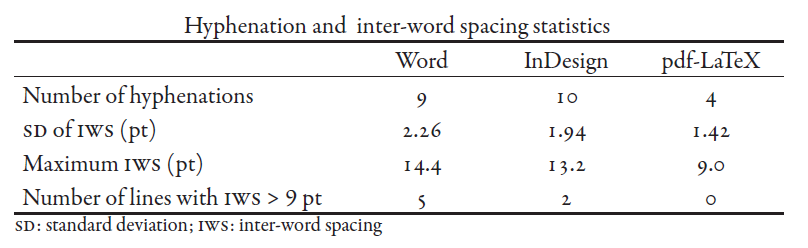
\includegraphics[width=0.6\textwidth]{twcomp2}
    
    \skfootnote{\stExC{https://tex.stackexchange.com/questions/110133/visual-comparison-between-latex-and-word-output-hyphenation-typesetting-ligat} \url{http://www.rtznet.nl/zink/latex.php?lang=en}}
\end{frame}


\begin{frame}\relax
    \Huge\centering ``this, in fact, is probably the most interesting aspect of the whole TEX system''\\\hfill \large D. Knuth, the \TeX Book

\end{frame}

\begin{frame}{Paragraph creation overview\preMagicPage}\relax
    \begin{itemize}
        \item All paragraph is considered as one: the words in the last line can change the typesetting in the first line.
        \item \TeX\ will never put words narrow than the glue allow.
        \item \TeX\ tries out all possible varients for line breaks. For each varient and each line \TeX\ calculates the \textit{badness}. If it is lower than \ccol\tolerance, \TeX\ will try to create paragraph with the minimum of hyphenation.
        \item if \TeX\ fails, it provides \textbf{Overfull} or \textbf{Underfull} warnings.
    \end{itemize}
    \skfootnote{\knuthc{14}[101] \lvoc{3.6}[114] \lmanc{9}[100]}
\end{frame}

\begin{frame}[fragile]{How to suggest a hyphentation\magicPage}\relax

    Locally: use \ccol\- \verb|as in this ve\-ry long se\-nta\-nce|
    
    Globally: \ccol\hyphenation\verb|{some-thing poss-ible}|
    
    \cprotect\skfootnote{\ccol\- is just a short version for \ccol\discretionary\verb|{hpre-break texti}{hpost-break texti}{hno-break texti}|\\ 
    also: \TeX\ will never hyphenate the word with ``/''. Use \ccol\slash if you want to allow it. And \ccol\uchyph=0 will prohibit hyphenation in words on uppercase letter.}
\end{frame}

\begin{frame}{Manual line break manipulation\magicPage}\relax

    Never break: non-breaking space \verb|~|, \ccol\nobreak, \ccol\nolinebreak
    
    Always: \ccol\\, \ccol\break, \ccol\linebreak
    
    You can use \ccol\obeylines\ to follow the line breaks in the source code.
     
     \skfootnote{by the way: \ccol\\ \ has an optional parameter: the vertical space after the command. Also \ccol\smallskipamount, \ccol\medskipamount\ and \ccol\bigskipamount\ responsible for skipping after paragraph. \ccol\linebreak\ has an optional parameter: [0-4] how much you want to have the break here.}
\end{frame}

\begin{frame}{Algorithm: part 1\magicPage}\relax
    
    \begin{enumerate}
        \item \TeX\ produce varients without word breaks. It compare the \textit{badness} with \ccol\pretolerance\ param. 
        \item \textit{badness} is $\simeq$ 100$\cdot$<proportion-between-the-normal-glue-and-its-stretching/compression>$^3$
        \item if \ccol\pretolerance-try fall, \TeX will try to use all posible line breaks to make each badness less than \ccol\tolerance
         
    \end{enumerate}
     
     \skfootnote{defaults: \ccol\pretolerance=100, \ccol\tolerance=200. \ccol\pretolerance>=10000, the first try will always succeed}
\end{frame}

\begin{frame}{Algorithm: part 2\magicPage}\relax

    \begin{enumerate}
        \item line breaks are allowed only in certain places:
        \begin{enumerate}
            \item glue
            \item kern with glue after 
            \item and of math (\$) and glue after 
            \item the manual or auto-passed penalty
            \item  discretionary break
        \end{enumerate}
        \item The penalty to the first three is $0$. For the last one, it is defined by \ccol\hyphenpenalty=\ or \ccol\exhyphenpenalty=. The penalty can be manually added as \ccol\penalty
        \item Penalty can both positive and negative. If it is $>10^4$ there will be no break ever, if it is $<-10^4$ there always will be a break
         
    \end{enumerate}
         
    \skfootnote{defaults: \ccol\hyphenpenalty=50, \ccol\exhyphenpenalty=50\\ 
you can put addition spaces between math and text with \ccol\mathsurround}
\end{frame}


\begin{frame}{Algorithm: part 3\magicPage}\relax
    
    \begin{enumerate}
    \item in reality, \TeX\ tries to minimize the \textit{demerits}. It is proportional to the {\csk badnesses}, \ccol\linepenalty (determines how much you want tex to produce a minimum amount of lines) and {\csk penalty}
    \item \TeX\ also takes into account and add penalty if two lines one after another has a hyphenation (\ccol\doublehyphendemerits), if lines are \textit{visually incompatible} (ex: if a tight line is next to a loose one) (\ccol\adjdemerits) and if the second-last line of the entire paragraph ends with a discretionary (\ccol\finalhyphendemerits)
    
    \end{enumerate}
         
     \skfootnote{defaults: \ccol\linepenalty=10, \ccol\adjdemerits=10000, \ccol\doublehyphendemerits=10000, \ccol\finalhyphendemerits=5000.\\ 
     \ccol\hfuzz=... will add the maximum length of string's aligment}
\end{frame}

\begin{frame}{What else? \magicPage}\relax 
    \def\strutdepth{\dp\strutbox}
    \def\marginalstar{\strut\vadjust{\kern-\strutdepth\specialstar}}
    \def\specialstar{\vtop to \strutdepth{
    \baselineskip\strutdepth
    \vss\llap{* }\null}}
    
    \begin{itemize}
        \item Use \ccol\narrow\ to make lines narrow
        \item Use \ccol\looseness=-1 to ask \TeX\ to try make one line less in paragraph
        \item \ccol\prevgraf\ shows the curent line in the paragraph.
        \item \ccol\vadjust\ adds something at the vertical list after current line. With it we add the star to the left \marginalstar
        \item \ccol\everypar adds something in each paragraph
        \item \ccol\parfillskip --- the glue after last line 
        \item \ccol\parskip --- the vertical glue between paragraphs
         
    \end{itemize}
     
\end{frame}

\begin{frame}{Non-standart paragraph form\magicPage}\relax
    \twocolImg{
    % \lstinputlisting[linerange={13-21}]{handmy.tex}
    \inputminted[firstline=13, lastline=21]{latex}{sec/code/handmy.tex}
    }{handmy}
    \footnotesize
    \ccol\hangindent=[>0] --- the addition indent to the left. ...=[<0] --- indent to the right.
    
    \ccol\hangafter=[>0] --- the indent to all lines after. ...=[<0] --- before.
    \end{frame}
    
    \begin{frame}{Non-standart paragraph form\magicPage}\relax
    \twocolImg{
    % \lstinputlisting[linerange={13-19}]{parshapemy.tex}
    \inputminted[firstline=13, lastline=19]{latex}{sec/code/parshapemy.tex}
    }{parshapemy}
\end{frame}


\begin{frame}{Page creation}
    \begin{itemize}
        \item \TeX\ was created in time when it was not enough memory to optimize pages globally.
        \item \TeX\ finds the best break to the current page and then erase it from memory.
        \item More or less the algorithms are the same.
        \item You can use \ccol\penalty\ or \ccol\nobreak\ in vertical mode
        \item You can use \raggedbottom\ to remove bottom page alignment 
        \item Also as in paragraph, you allow to use \ccol\newpage, \ccol\pagebreak, \ccol\nopagebreak
         
    \end{itemize}
     
     \skfootnote{\knuthc{15}[119] \lvoc{III.9}[141] \lmanc{10}[105]}
\end{frame}
